\section{Auswertung}

Bei der Nullmessung wurde ein Zeitintervall von $\increment t = 900$ gewählt und
es wurden zwei Messungen durchgeführt, deren Mittelwert für weitere Berechnungen
verwendet wurde:

\begin{align*}
  N\ua{1} &= 218 \\
  N\ua{2} &= 224 \\
  \bar{N} &= 221 \\
  \sigma\ua{Nullmessung} = 14.87
\end{align*}

Bei allen Messungen wird eine lineare Regression in der folgenden Form verwendet,
um die Zerfallskonstante zu bestimmen:

\begin{equation}
  f(x) = A \cdot x + B
  \label{eqn:linRegress}
\end{equation}

\subsection{Halbwertszeit von Indium}

Bei der Messung von Indium wurde ein Zeitintervall von $\increment t = 240 \,
\su{s}$ und ein Messzeitraum von $t\ua{ges} = 3600 \, \su{s}$ gewählt. Die
gemessenen Zerfälle sind in Tabelle \ref{tab:Indium} eingetragen und grafisch
in Abbildung \ref{fig:Indium} dargestellt.

\begin{table}
  \centering
  \caption{Gemessene Zerfälle bei Indium.}
  \label{tab:Indium}
  \begin{tabular}{c c c c}
    \toprule $\increment t \, in \, \su{s}$ & $Anz. \, Zerfaelle$ & $\increment t \, in \, \su{s}$ & $Anz. \, Zerfaelle$ \\
    \midrule
    240 & 2995  & 480  & 2485 \\
    720 & 2465  & 960  & 2346 \\
    1200 & 2345 & 1440 & 2268 \\
    1680 & 2076 & 1920 & 1943 \\
    2160 & 1894 & 2400 & 1827 \\
    2640 & 1686 & 2880 & 1555 \\
    3120 & 1525 & 3360 & 1512 \\
    3600 & 1417 &      &      \\
    \bottomrule
  \end{tabular}
\end{table}

\begin{figure}
  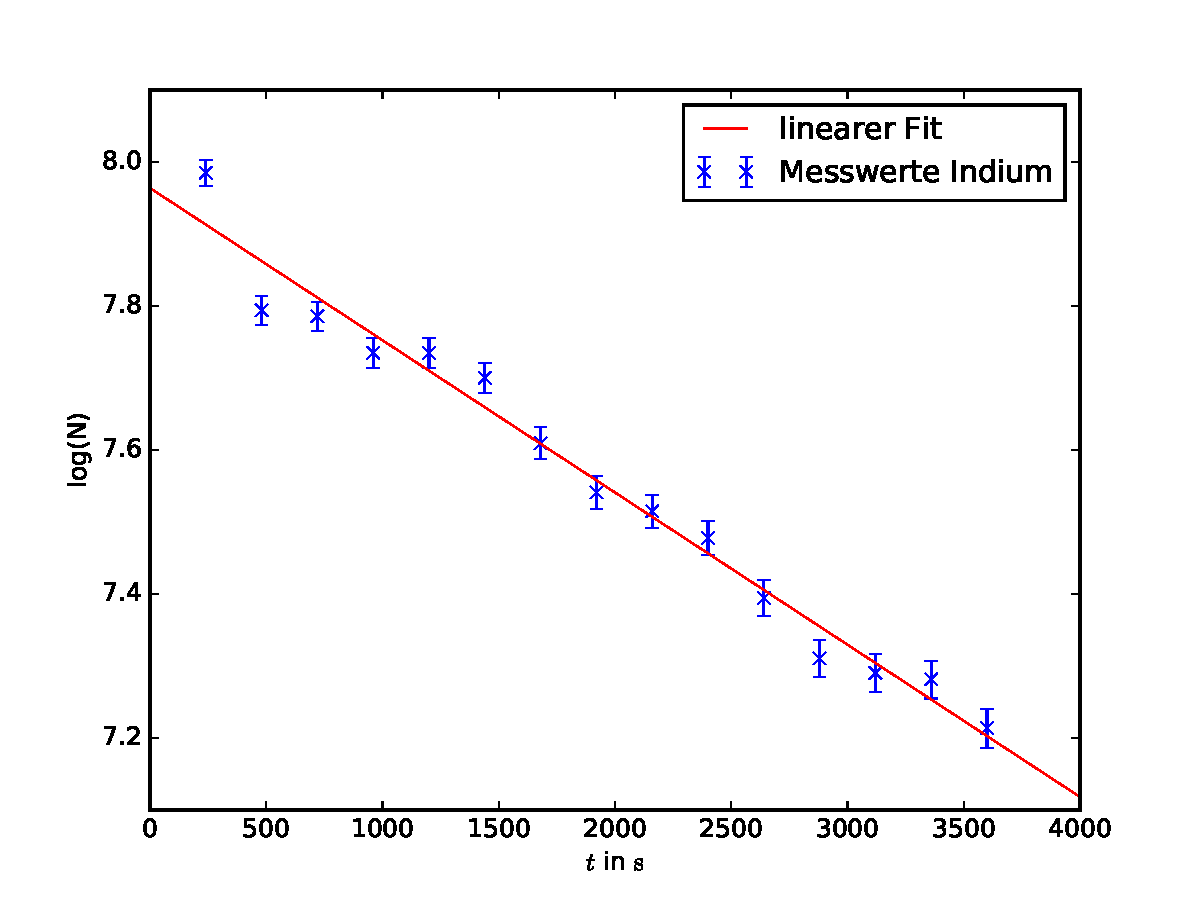
\includegraphics[width = \textwidth]{Indium_log.pdf}
  \caption{logarythmische Darstellung der gemessenen Zerfälle bei Indium.}
  \label{fig:Indium}
\end{figure}

Mithilfe einer linearen Regression der Form \eqref{eqn:linRegress} gemäß Formel
\eqref{eqn:expo} werden dabei die Zeitkonstante $\lambda$ und $N\ua{0,Indium}$ bestimmt:

\begin{align*}
A &= \lambda\ua{Indium} = (0.0002 \pm 9 \cdot 10^{-6}) \, \frac{1}{\su{s}}\\
B &= N\ua{0,Indium}     = (7.96 \pm 0.02)
\end{align*}

\begin{align}
  T(\lambda) &= \frac{ln(2)}{\lambda} \\
  \sigma_{T} &= \frac{ln(2)}{\lambda^2} \cdot \sigma_{\lambda}
  \label{eqn:Halbwert}
\end{align}


Mit der Formel \eqref{eqn:Halbwert} kann aus der bestimmten Zeitkonstante nun die Halbwertzeit von
Indium bestimmt werden, für die sich der folgende Wert ergibt:

\begin{equation*}
  T\ua{Indium} = (3278 \pm 141) \, \su{s}
\end{equation*}

\subsection{Halbwertzeit von Rhodium}

Bei der Messung mit $\su{Rh}_{45}^{103}$ wurde ein Zeitintervall von $\increment t = 12 \,
\su{s}$ und ein Messzeitraum von $t\ua{ges} = 720 \, \su{s}$ gewählt. Die gemessenen
Zerfälle sind in Tabelle \ref{tab:Indium} eingetragen sowie grafisch in Abbildung
\ref{fig:RhodiumOhne} dargestellt.

\begin{table}
  \centering
  \caption{Gemessene Zerfälle bei Indium.}
  \label{tab:Indium}
  \begin{tabular}{c c c c c c}
    \toprule $\increment t \, in \, \su{s}$ & $Anz. \, Zerfaelle$ & $\increment t \, in \, \su{s}$ & $Anz. \, Zerfaelle$
           & $\increment t \, in \, \su{s}$ & $Anz. \, Zerfaelle$ \\
    \midrule
    15 & 630 & 30 & 517 & 45 & 445 \\
    60 & 330 & 75 & 265 & 90 & 212 \\
    105 & 192 & 120 & 176 & 135 & 152 \\
    150 & 116 & 165 & 99 & 180 & 98 \\
    195 & 92 & 210 & 64 & 225 & 55 \\
    240 & 60 & 255 & 55 & 270 & 61 \\
    285 & 51 & 300 & 51 & 315 & 33 \\
    330 & 40 & 345 & 48 & 360 & 28 \\
    375 & 32 & 390 & 35 & 405 & 33 \\
    420 & 25 & 435 & 22 & 450 & 29 \\
    465 & 18 & 480 & 27 & 495 & 22 \\
    510 & 22 & 525 & 25 & 540 & 25 \\
    555 & 22 & 570 & 20 & 585 & 22 \\
    600 & 13 & 615 & 24 & 630 & 23 \\
    645 & 12 & 660 & 21 & 675 & 19 \\
    690 & 18 & 705 & 15 & 720 & 14 \\
    \bottomrule
  \end{tabular}
\end{table}

\begin{figure}
  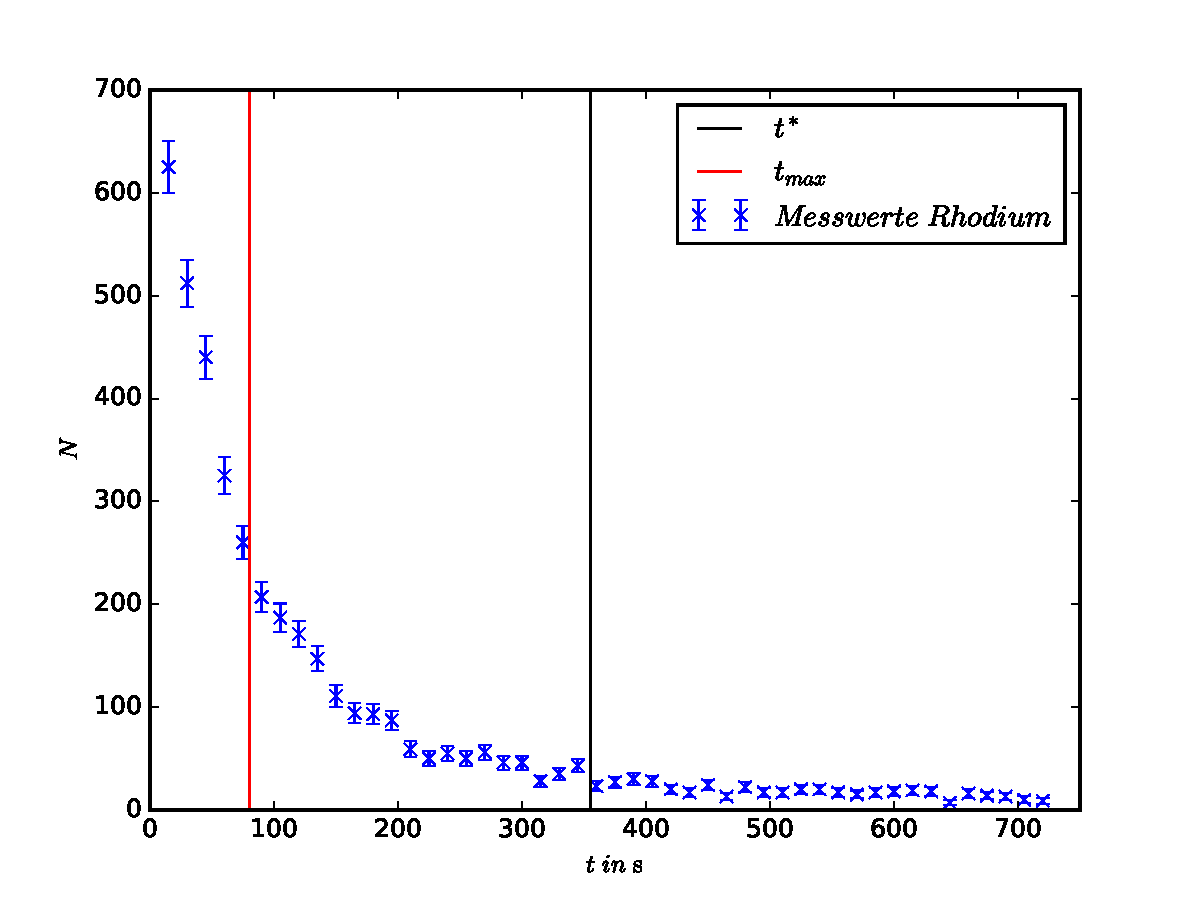
\includegraphics[width = \textwidth]{Rhodium_normal_ohne.pdf}
  \caption{Gemessene Zerfälle bei Rhodium.}
  \label{fig:RhodiumOhne}
\end{figure}

Um die Halbwertzeiten der zwei verschiedenen Isotope $\su{Rh}^{104}$ sowie $\su{Rh}^{104i}$
zu bestimmen, die bei dem Zerfall von $\su{Rh}_{45}^{103}$ entstehen, werden für die
Unterteilung die Messzeiten $t^{*}=355 \, \su{s}$ und $t_{max}=80 \, \su{s}$ gewählt.

\begin{figure}
  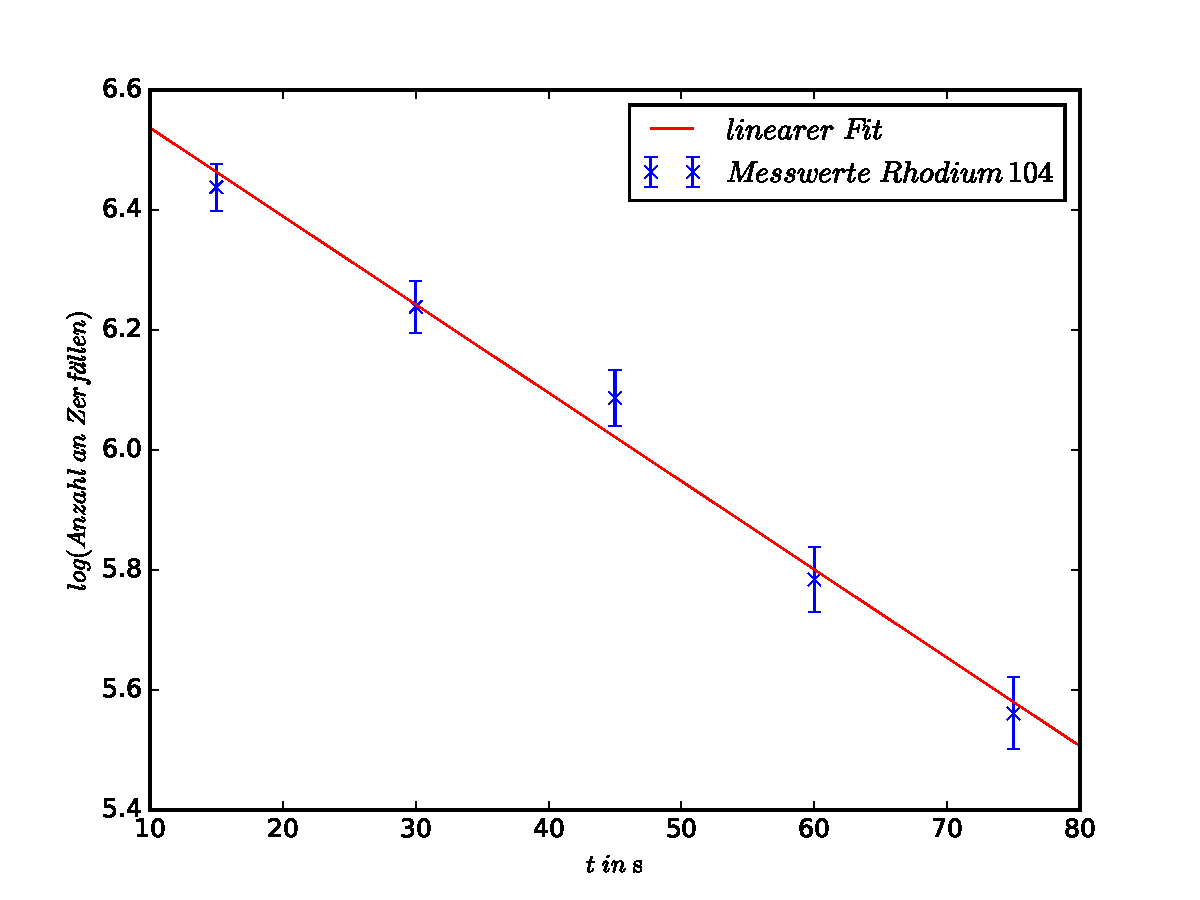
\includegraphics[width = \textwidth]{Rhodium_links_log.pdf}
  \caption{logarythmische Darstellung der gemessene Zerfälle für $t < t_{max}$ bei $\su{Rh}^{104}$.}
  \label{fig:Rh104}
\end{figure}

Mithilfe einer linearen Regression gemäß Formel \eqref{eqn:linRegress} können
dann mithilfe der Werte für $t < t_{max}$ (Abbildung \ref{fig:Rh104}) zuerst die beiden Parameter
für $\su{Rh}^{104}$ bestimmt werden:

\begin{align*}
  A &= \lambda\ua{Rhodium\,104} = (0.0147 \pm 0.0009) \, \frac{1}{\su{s}}\\
  B &= N\ua{0,Rhodium\,104}     = (6.68 \pm 0.05)
\end{align*}

Mit den Werten und Formel \eqref{eqn:Halbwert} ergibt sich für die Halbwertszeit
von $\su{Rh}^{104}$ folgender Wert:

\begin{equation*}
  T\ua{Rhodium\,104} = (47 \pm 3) \, \su{s}
\end{equation*}

Mithilfe der selben Vorgehensweise kann aus allen Werten für $t > t^{*}$ (Abbildung
\ref{fig:Rh104i}) auch die Halbwertszeit für $\su{Rh}^{104i}$ berechnet werden,
sodass sich folgende Parameter ergeben:

\begin{align*}
  A                  &= \lambda\ua{Rhodium\,104i} = (0.0023 \pm 0.0004) \, \frac{1}{\su{s}}\\
  B                  &= N\ua{0,Rhodium\,104i}     = (4.1 \pm 0.2) \\
  T\ua{Rhodium\,104i} &= (297 \pm 54) \, \su{s}
\end{align*}

\begin{figure}
  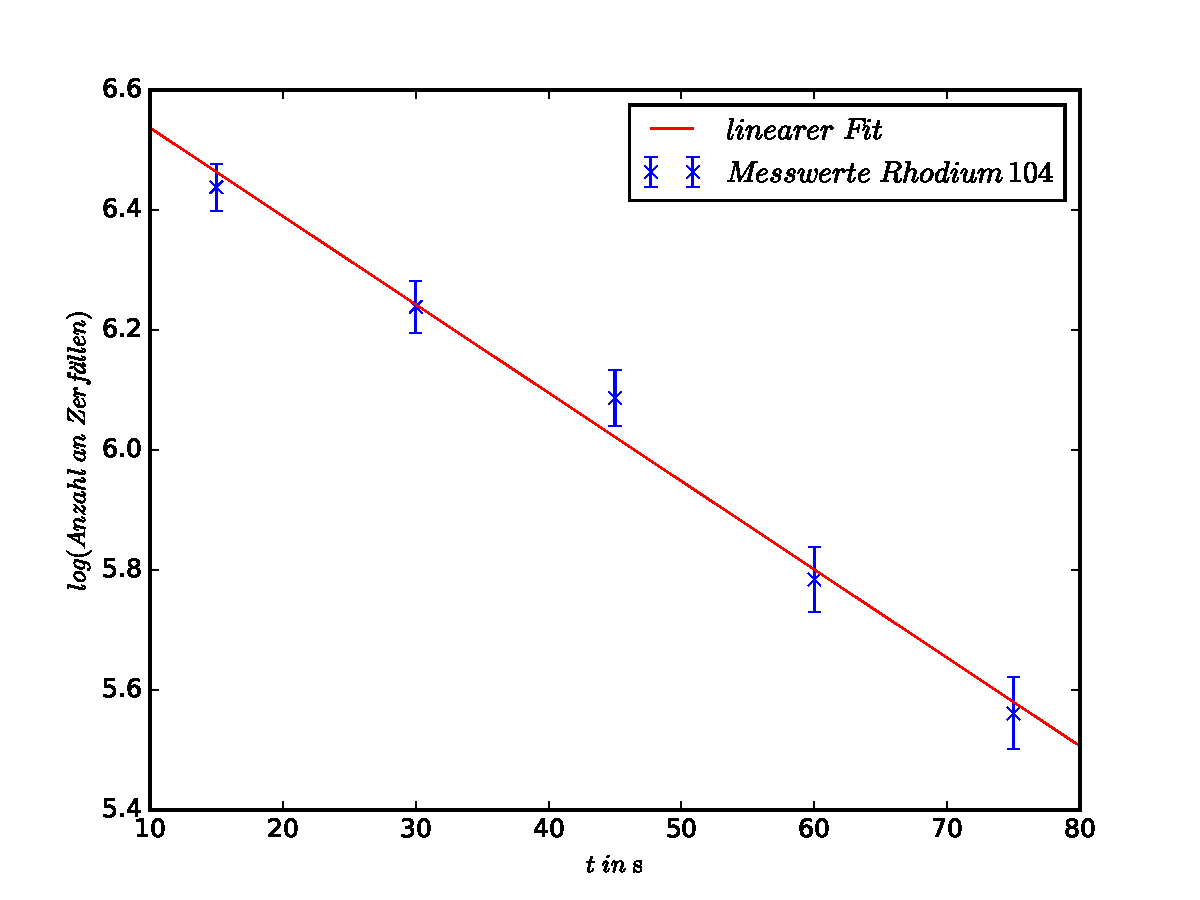
\includegraphics[width = \textwidth]{Rhodium_links_log.pdf}
  \caption{logarythmische Darstellung der gemessene Zerfälle für $t > t^{*}$ bei $\su{Rh}^{104i}$.}
  \label{fig:Rh104i}
\end{figure}

Mit den bestimmten Parametern für $\su{Rh}^{104}$ und $\su{Rh}^{104i}$ kann nun
auch eine Summenkurve nach Formel ?? gezeichnet werden (Abbildung \ref{fig:Summe}).

\begin{figure}
  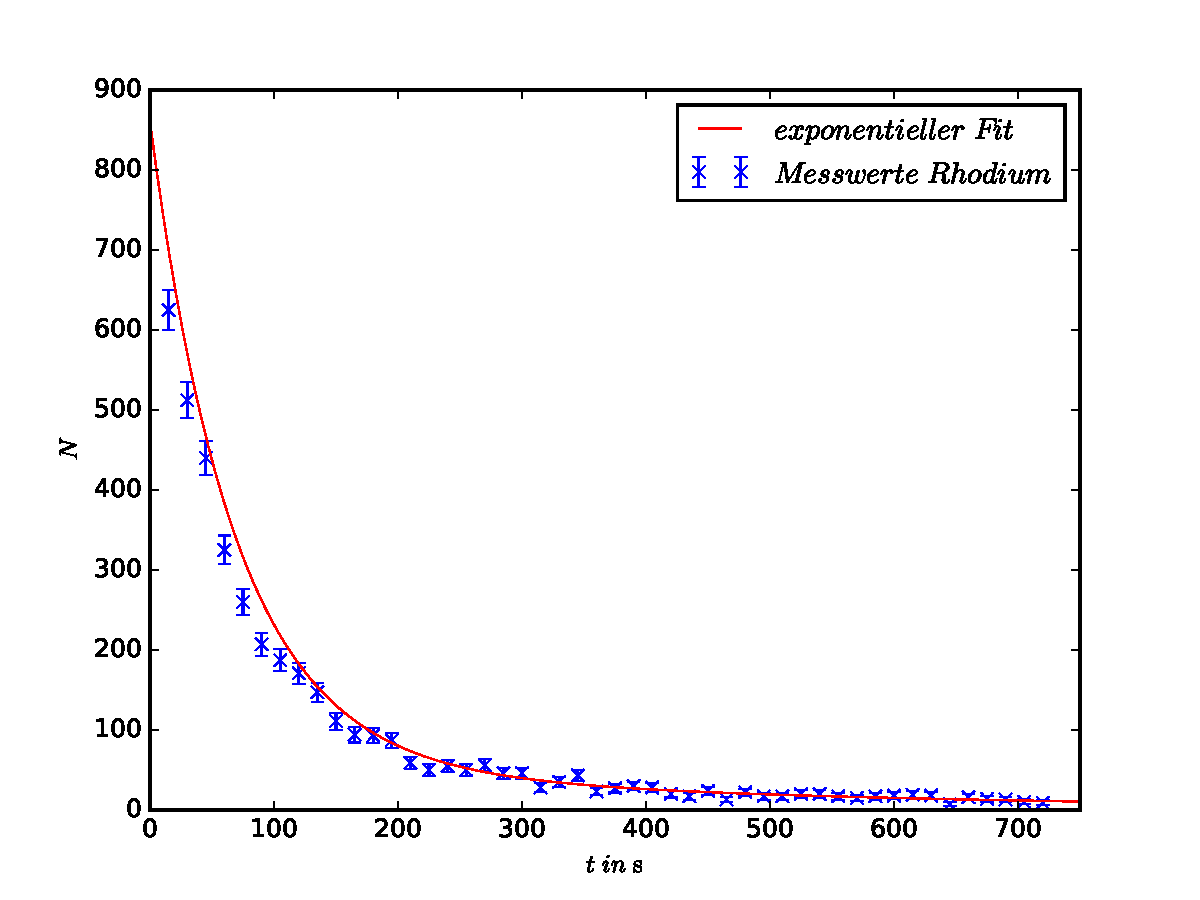
\includegraphics[width = \textwidth]{Rhodium_normal}
  \caption{Summenkurve für den Zerfall von $\su{Rh}_{45}^{103}$.}
  \label{fig:Summe}
\end{figure}

\newpage

\subsection{Diskussion}

Wenn man die berechneten Halbwertszeiten für $\su{Rh}_{45}^{103}$ und $\su{In}_{49}^{115}$
mit den Literaturwerten vergleicht, sieht man eine leichte Abweichung. Jedoch liegen
die Literaturwerte bei zweien der drei Isotope im Fehlerintervall des jeweiligen
experimentellen Werts und lediglich bei $\su{Rh}^{104}$ weicht der Wert stärker
ab (siehe Tabelle \ref{tab:vergleich}).

\begin{table}
  \centering
  \caption{Halbwertszeiten der verschiedenen Isotope \cite{Page01}.}
  \label{tab:vergleich}
  \begin{tabular}{c c c}
    \toprule
    Isotop & $T_{exp} \, in \, \su{s}$ & $T_{Lit} \, in \, \su{s}$ \\
    \midrule
    $\su{In}_{49}^{115}$ & $3278 \, \pm \, 141$ & $3269$ \\
    $\su{Rh}^{104}$      & $47 \, \pm \, 3$     & $42.3$ \\
    $\su{Rh}^{104i}$     & $297 \, \pm \, 54$   & $274$  \\
    \bottomrule
  \end{tabular}
\end{table}

Zusammen mit dieser Erkenntnis und den verschiedenen Abbildungen lässt sich darauf
schließen, dass die auftretenden Abweichungen lediglich durch statistische Fehler
hervorgerufen werden.

Fehlerquellen können hierbei vor allem der Nulleffekt und das Geiger-Müller-Zählrohr
sein, da die von der Umgebung abgegebene Radioaktivität im Laufe des Experimentes
schwankt und nicht anhand einer vorher ausgeführten Nullmessung komplett
eliminiert werden kann.
